% arara: pdflatex: { shell: true, draft: true }
% arara: makeglossaries
% arara: biber
% arara: pdflatex: { shell: true, synctex: true }
% arara: pdflatex: { shell: true, synctex: true }

\documentclass{f4_beamer_metropolis}

\title{Test-Driven Development in Scrumentwicklung}
\subtitle{PMQM WS18/19}
\author{Dennis Grabowski, B.Sc}
\date{17.11.2018}

\bibliography{./literature.bib}

\begin{document}

% Cannot be moved into the class
\begin{frame}{Inhaltsverzeichnis}
    \tableofcontents[hideallsubsections]
  \end{frame}

% P. 262-263, 490, 506, 5, 113 - 114, 111, 244-245, 237, 487
\section{Test-Driven Development}

\begin{frame}{Definition}
  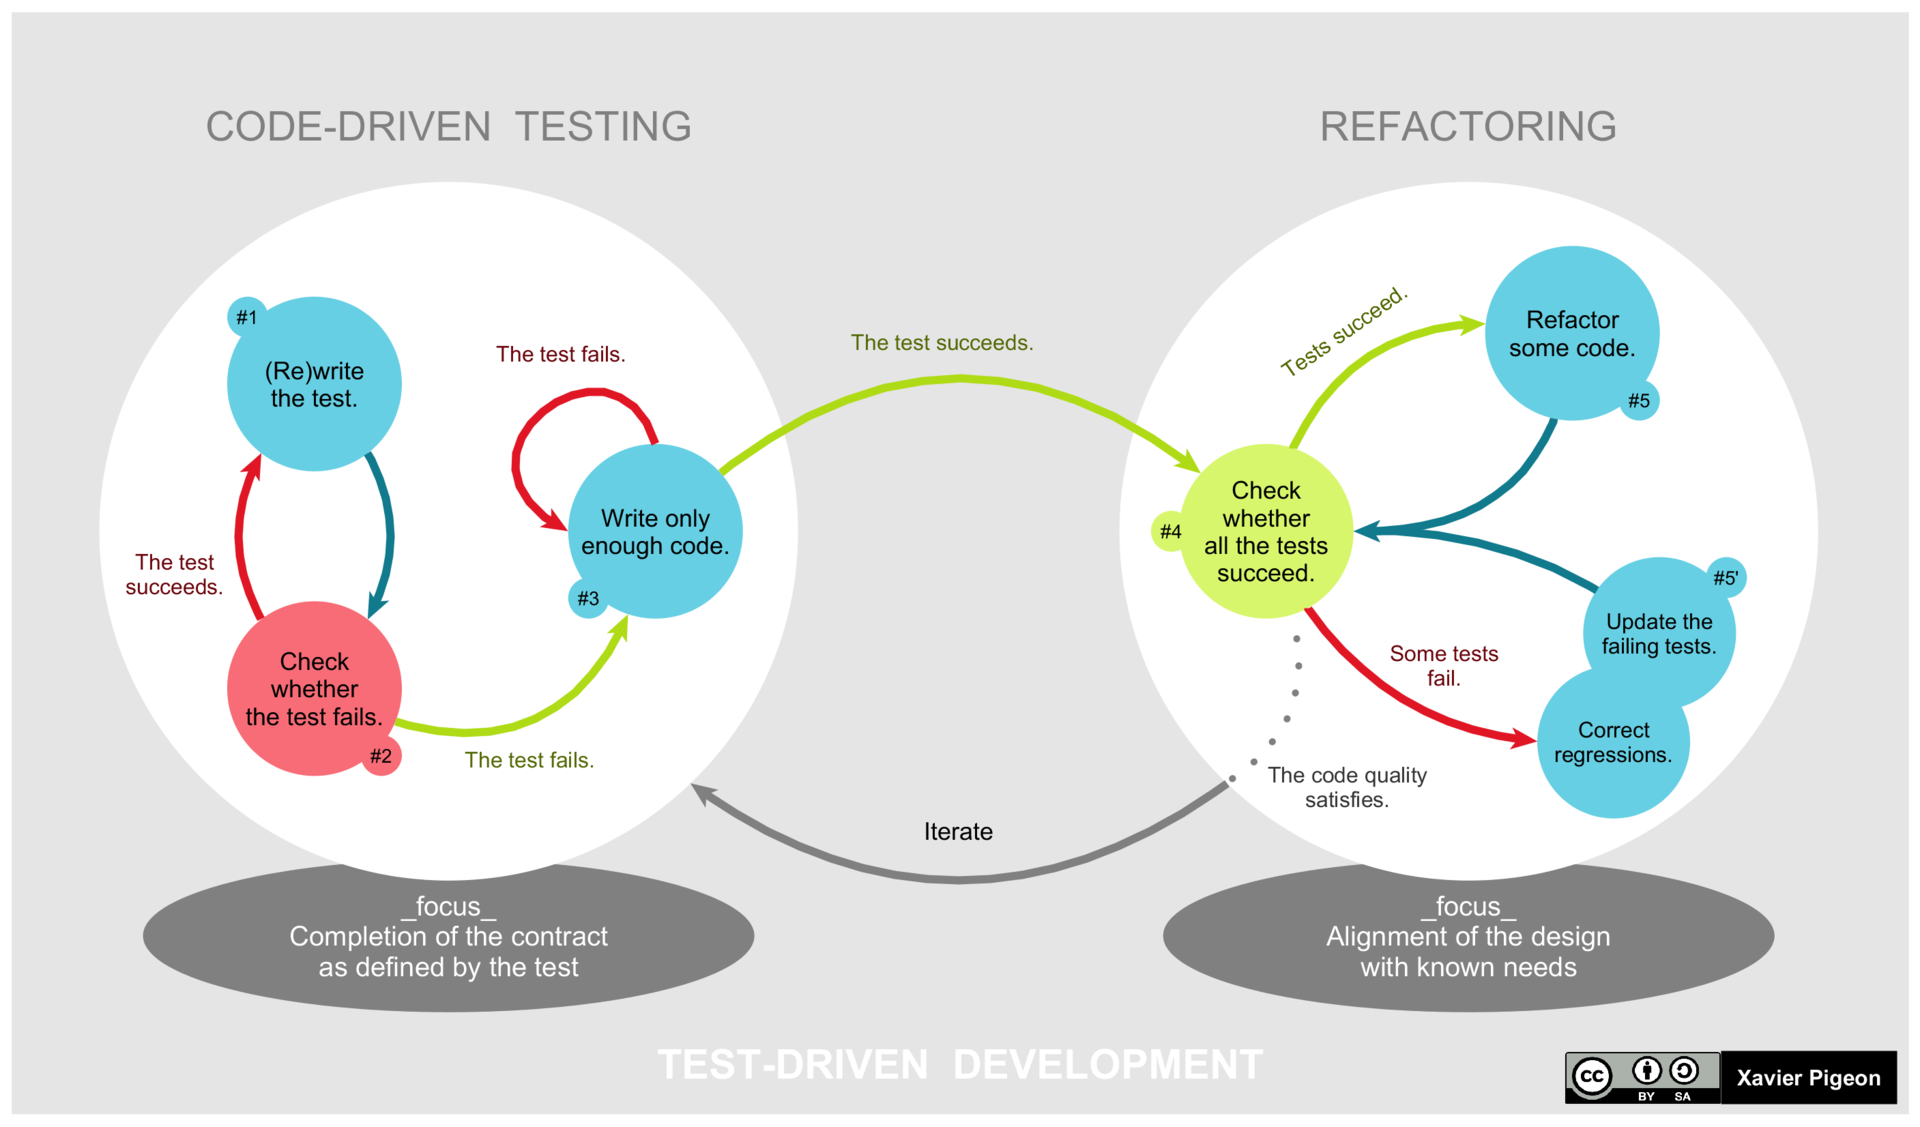
\includegraphics[width=\textwidth,height=0.85\textheight,keepaspectratio]{./images/1920px-TDD_Global_Lifecycle.png}
  \nocite{TDD.Picture}
\end{frame}

\section{Scrum}

\subsection{Übersicht}

\begin{frame}{Kernidee}
  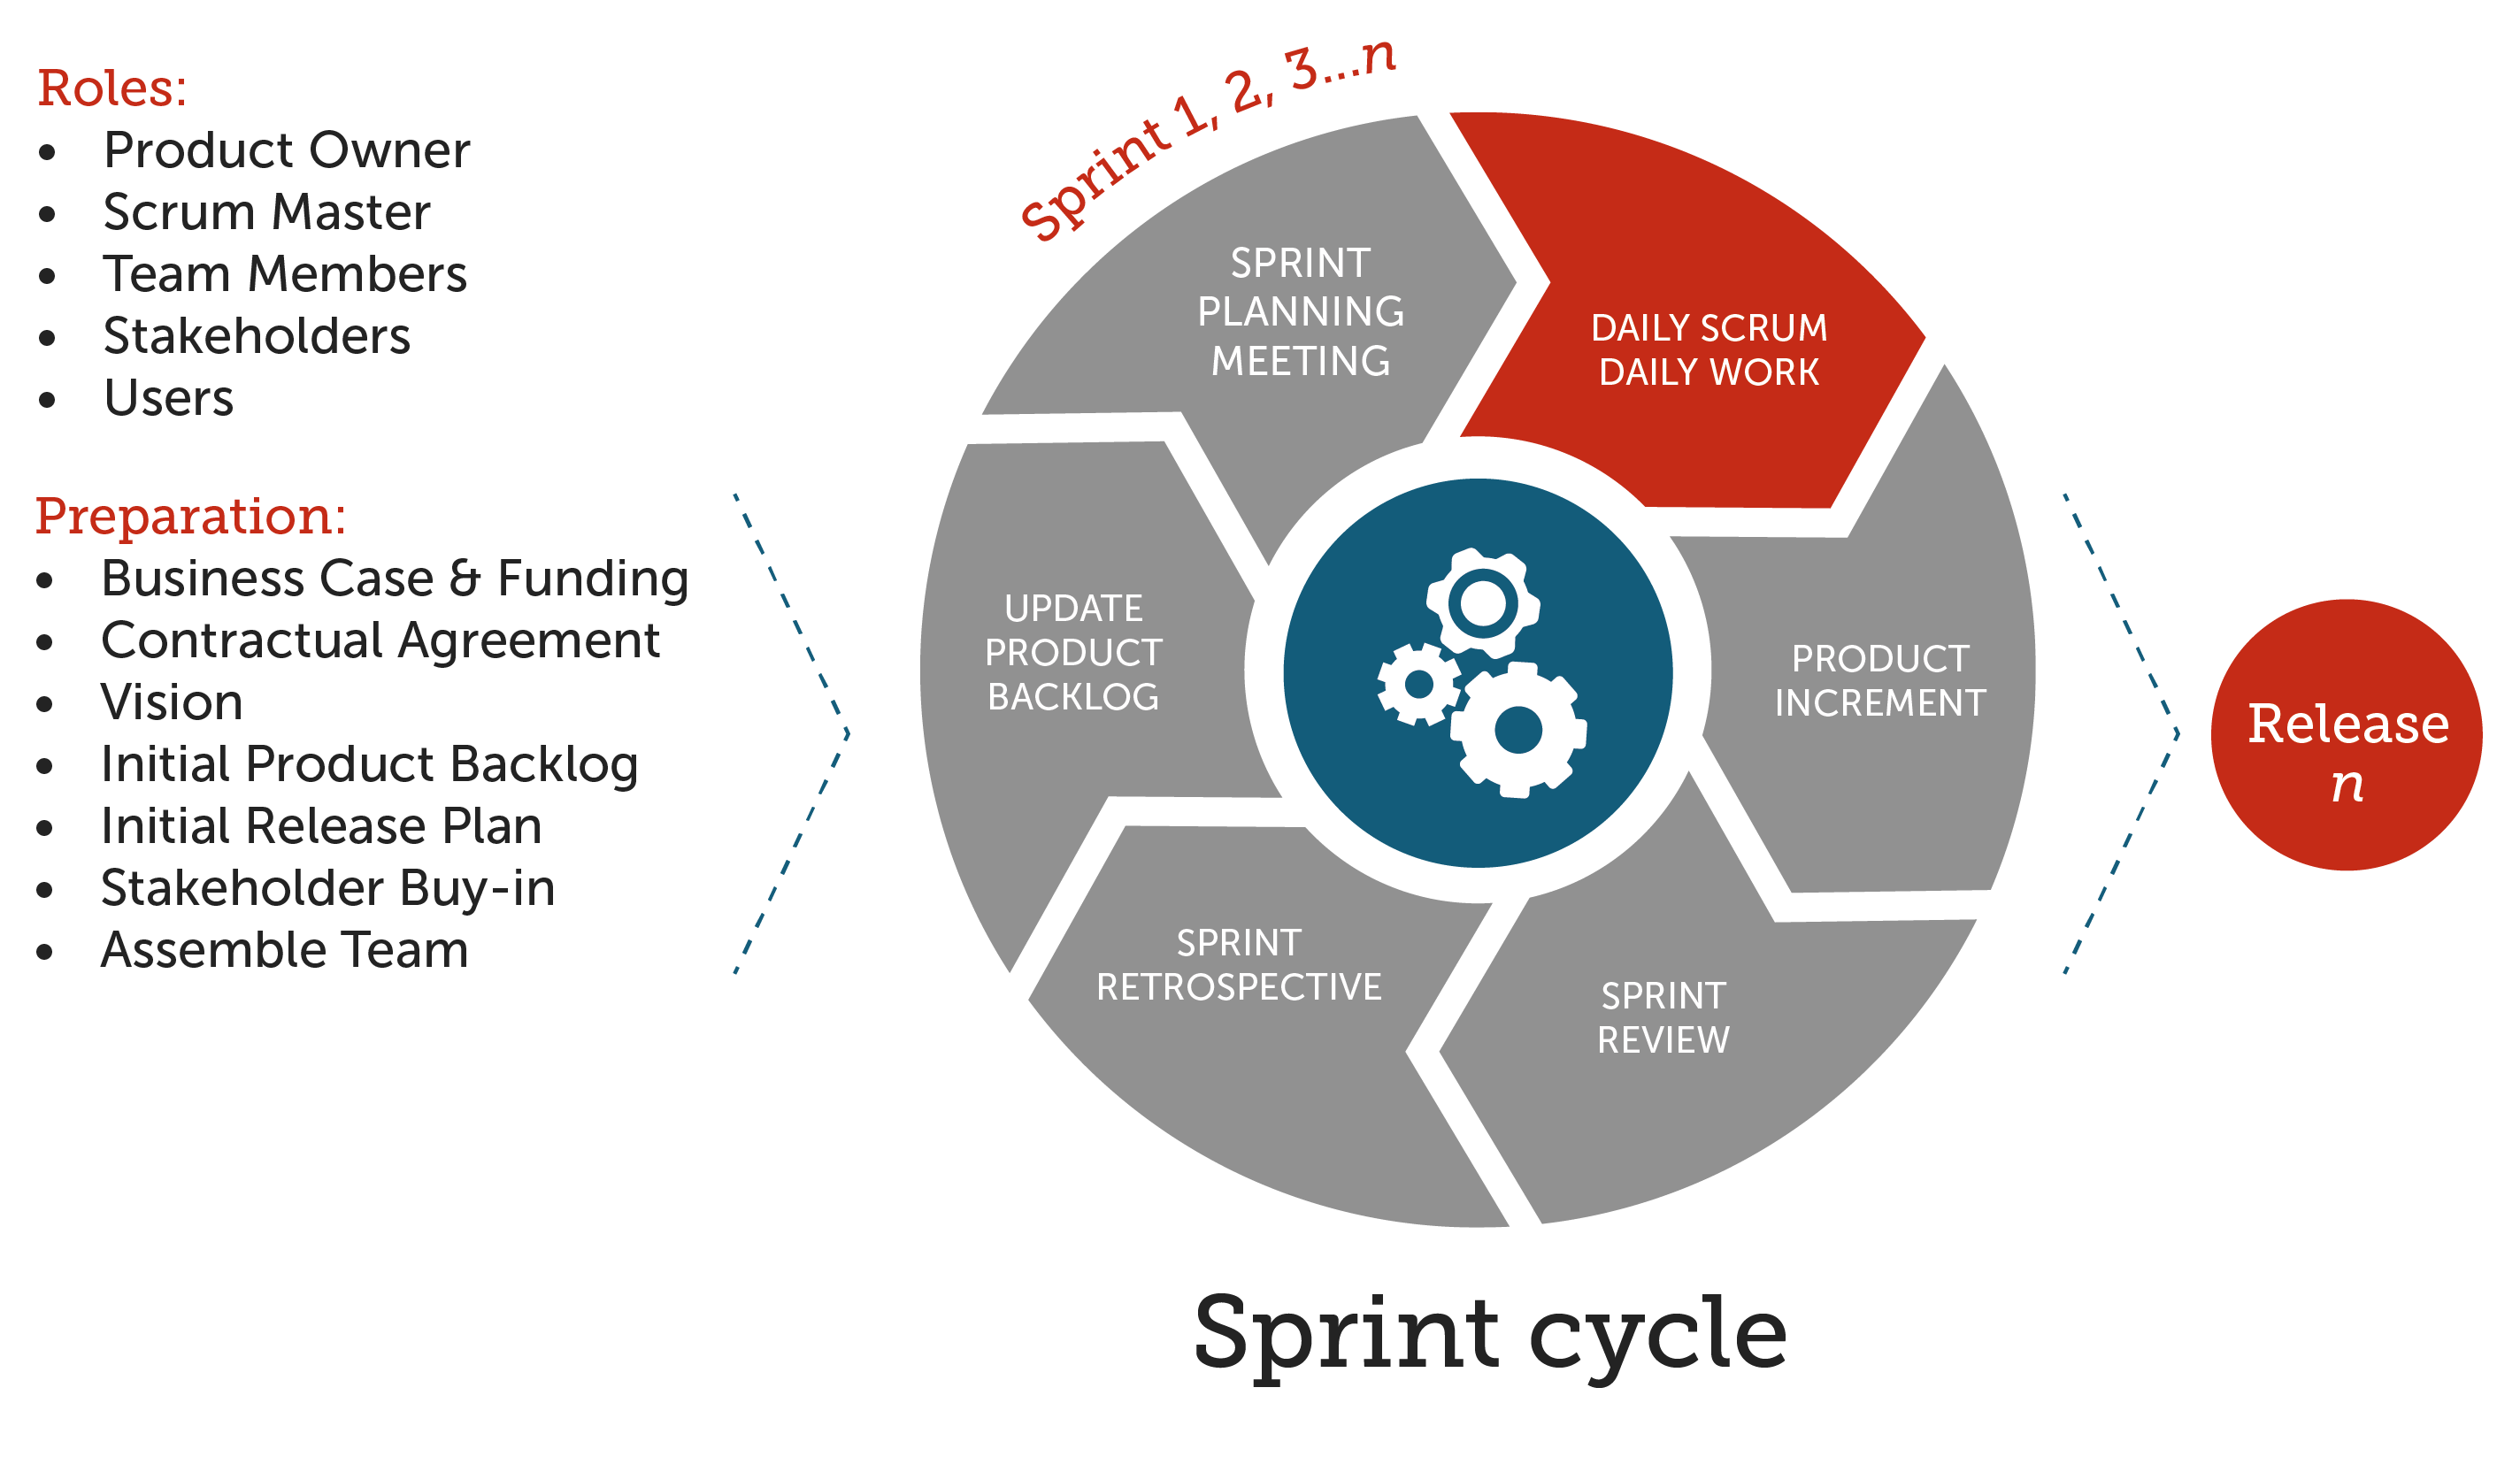
\includegraphics[width=\textwidth,height=0.9\textheight,keepaspectratio]{./images/the-daily-scrum-in-the-sprint-cycle}
  \nocite{ManifestoDigital}
\end{frame}

\subsection{Argumente für \& gegen Scrum}

\begin{frame}{Vorteile}
Sprint, Sprint Planning, Sprint Retrospective, Sprint Review, Daily Scrums - was bringt uns das alles?
\begin{itemize}
  \item Agilität
  \item Feedback durch Kommunikation zwischen allen Stakeholdern
  \item Iterative Natur
  \item Kostensparender Entwicklungsprozess
  \item Whole-Team-Approach
\end{itemize}
\note{
  Projekte mit vielen \enquote{moving targets} sind durch Scrum lösbar.
  Iterative Natur bietet Möglichkeit, Software schnell und strukturiert zu entwickeln, um ein Minimum Viable Project zu liefern.
  Kurzen Sprints erlauben, dass Software nicht für Ewigkeiten entwickelt wird, und dann ein falsches Projekt herauskommt.
  Probleme werden schnell identifiziert.
  Planung von Sprint zu Sprint, Team organisiert sich selbst, daher wenig Overhead.
  Nur Features implementiert, die der Kunde explizit fordert
}
\end{frame}

\begin{frame}{Nachteile}
  \begin{itemize}
    \item Nur ein Framework
    \item Kein festes Projektabschlussdatum führt oft zu \enquote{Feature Creep}
    \item Keine festen Softwareentwicklungsphasen innerhalb eines Sprints
    \item Projekterfolg hängt von Kooperation des Teams ab
    \item Erfordert viel Disziplin
    \item Qualität schwer zu gewährleisten:
    \begin{itemize}
      \item Team muss entweder qualifiziert sein oder
      \item Team muss agressiven Testprozess durchführen
    \end{itemize}
  \end{itemize}

  \note{Anforderungserhebung, Anforderungsanalyse, Design, Entwicklung Testing, Deployment...}
\end{frame}

\section{Zusammenführung beider Techniken}

\begin{frame}{Zentrale Fragen bei der Softwareentwicklung}
Barry Boehm (Erfinder des Spiralenmodells) hat Unterschied schön hervorgehoben: \\
\textbf{Verifikation:} \\
\only<2-3>{\enquote{Are we building the product right?}} \\
\textbf{Validierung:} \\
\only<3>{\enquote{Are we building the right product?}}

  \note{Validation abgedeckt durch Scrums Sprint Planning und Füllen des Product Backlogs}
  \end{frame}

  \subsection{Statistiken}
  \begin{frame}{Wie verifizieren agile Teame ihre Arbeit?}
      \begin{tabularx}{\linewidth}{
        |>{\hsize=0.7\hsize} X |
        >{\hsize=0.2\hsize} X |
        >{\hsize=0.1\hsize} X |
        >{\hsize=0.1\hsize} X |
      }
      \hline
      \textbf{Methodik} & \textbf{2008} & \textbf{2010} & \textbf{2013}\\ \hline
      Iteration demos & - & \textbf{79\%} & 58\% \\ \hline
      Developer regression testing & 60\% & \textbf{71\%} & 49\% \\ \hline
      Developer TDD & \textbf{71\%} & 53\% & 38\% \\ \hline
      Acceptance TDD & 40\% & \textbf{44\%} & 18\% \\ \hline
      All-hands demos & \textbf{56\%} & 42\% & 30\% \\ \hline
      End-of-lifecycle testing & 45\% & 41\% & \textbf{50\%} \\ \hline
      Non-solo development & - & \textbf{39\%} & 34\% \\ \hline
      Static-code analysis & - & 32\% & \textbf{39\%} \\ \hline
      Parallel independent testing & \textbf{36\%} & 26\% & 22\% \\ \hline
      External reviews & \textbf{52\%} & 23\% & 32\% \\ \hline
      Dynamic code analysis & \textbf{23\%} & 21\% & 22\% \\ \hline
      \end{tabularx}
  \end{frame}

  \begin{frame}{Welche agile Testmethode waren die schwersten zu erlernen?}
    \begin{tabularx}{\linewidth}{
      |>{\hsize=0.7\hsize} X |
      >{\hsize=0.2\hsize} X |
      >{\hsize=0.1\hsize} X |
      >{\hsize=0.1\hsize} X |
    }
    \hline
    \textbf{Methodik} & \textbf{2009} & \textbf{2012}\\ \hline
    Developer TDD & 37\% & 37\% \\ \hline
    Acceptance TDD & 30\% & 39\% \\ \hline
    \end{tabularx}

  Nur 2012:
    \begin{itemize}
      \item Getting all testing done in current sprint: 50\%
      \item Validating non-functional requirements: 33\%
      \item Getting stakeholders/customers involved in testing: 33\%
      \item Getting developers to test their own code: 27\%
      \item Initial Estimate and Schedule: 26\%
      \item Adopting new agile testing tools: 16\%
      \item Learning to test throughout the agile lifecycle: 16\%
    \end{itemize}
    \nocite{Ambysoft.Surveys}
  \end{frame}

\subsection{Wie passt TDD in Scrum?}

\begin{frame}{Offene Fragen}
\begin{itemize}
  \item Wird Code der jetzigen Sprint getestet?
  \item Wird Code der letzten Sprint getestet?
  \item Wann ist eine Story wirklich \enquote{done}? Alle Tests grün?
  \item Spezifikationen oftmals nicht genau - Können überhaupt ausreichend Tests geschrieben werden?
  \item Wer schreibt Tests?
\end{itemize}
\nocite{gregory_crispin_2015}
\end{frame}

\begin{frame}{Lücken in Scrum, die TDD füllt}
\begin{itemize}
  \item Explizite \enquote{Testphase} durch TDD
  \item \enquote{Definition of Done}: Tests inkl.
  \item Automatisierbare Tests, da kurze Entwicklungszyklen
\end{itemize}
\end{frame}

\subsection{Beispiel einer Integration von TDD in Sprint}

\begin{frame}{Developer-TDD + ATDD}
  \begin{itemize}
    \item Während Sprint Planning: Benutzeranforderungen als Acceptance Tests schreiben,
    \item Während User Stories: Acceptance Test aufgeteilt in kleinere Unit Tests,
    \item Eigentlicher Programmierprozess beginnt, bis Unit Tests / Acceptance Tests bestehen
  \end{itemize}
\end{frame}

\begin{frame}{Developer-TDD + ATDD}
  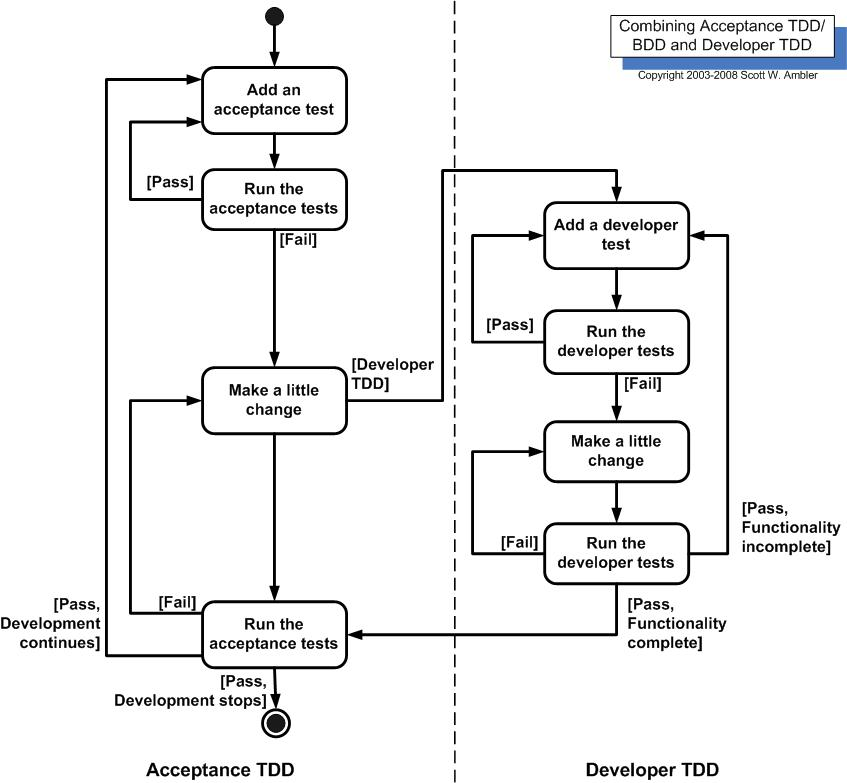
\includegraphics[width=\textwidth,height=0.8\textheight,keepaspectratio]{./images/atdd.jpg}
  \nocite{astels_2003}
\end{frame}

\begin{frame}[standout]
  Eigene Erfahrungen mit Testing in agilen Entwicklungsmethoden?
\end{frame}

\section{Konklusion}

\begin{frame}{Vorteile}
Vorteile von TDD gelten natürlich auch (Refactoring einfacher, sauberer Code...)
\begin{itemize}
  \item Tests bieten viel \textit{instant} Feedback
  \item Risikominderung:
  \begin{itemize}
    \item Schlechte Anforderungen können früher identifiziert werden
    \item \enquote{Technical Debt} kann früher abgebaut werden
    \item Änderungen am Code können besser aufgefangen werden
  \end{itemize}
  \item \enquote{Executable Specification}: implizite Dokumentation
\end{itemize}
\note{Tests ermöglichen, dass spätere Sprints nicht hauptsächlich Bugfixing sind}
\end{frame}

\begin{frame}{Nachteile}
\begin{itemize}
  \item Time Estimates der User Stories schwer für Entwickler
  \item Return on Investment schwer zu quantifizieren:
  \begin{itemize}
    \item Ist Code-Qualität wirklich höher mit TDD?
    \item Selbe Code-Qualität ohne TDD erreichbar?
  \end{itemize}
  \item Scrum benötigt bereits qualifiziertes Team - mit TDD höhere Qualifikation nötig?
  \item TDD deckt keine Usability, Performance oder andere "ility" Tests ab
  \item Whole-Team-Approach benötigt - 50\% des Teams reicht nicht
\end{itemize}
\note{Scalability, Availability/Reliability, Security, Accessability...}
\end{frame}

\begin{frame}{Zitate}
  \begin{displayquote}
  TDD misleads practitioners who do not understand that it's more about design than testing. \\
  Code developed test-first is naturally designed for testability.
  \\
  \\
  (Aus \enquote{\textbf{\citetitle{crispinlisa_gregoryjanet_2014}}}, \citeauthor{crispinlisa_gregoryjanet_2014})
  \end{displayquote}
\end{frame}

\begin{frame}[standout]
  Offene Fragen?
\end{frame}

\appendix

\section{Literatur}

\begin{frame}[allowframebreaks]{Literatur}
  \printbibliography
\end{frame}

\end{document}
